\documentclass[11pt,]{article}
\usepackage[left=1in,top=1in,right=1in,bottom=1in]{geometry}
\newcommand*{\authorfont}{\fontfamily{phv}\selectfont}
\usepackage[]{mathpazo}


  \usepackage[T1]{fontenc}
  \usepackage[utf8]{inputenc}



\usepackage{abstract}
\renewcommand{\abstractname}{}    % clear the title
\renewcommand{\absnamepos}{empty} % originally center

\renewenvironment{abstract}
 {{%
    \setlength{\leftmargin}{0mm}
    \setlength{\rightmargin}{\leftmargin}%
  }%
  \relax}
 {\endlist}

\makeatletter
\def\@maketitle{%
  \newpage
%  \null
%  \vskip 2em%
%  \begin{center}%
  \let \footnote \thanks
    {\fontsize{18}{20}\selectfont\raggedright  \setlength{\parindent}{0pt} \@title \par}%
}
%\fi
\makeatother




\setcounter{secnumdepth}{0}

\usepackage{color}
\usepackage{fancyvrb}
\newcommand{\VerbBar}{|}
\newcommand{\VERB}{\Verb[commandchars=\\\{\}]}
\DefineVerbatimEnvironment{Highlighting}{Verbatim}{commandchars=\\\{\}}
% Add ',fontsize=\small' for more characters per line
\usepackage{framed}
\definecolor{shadecolor}{RGB}{248,248,248}
\newenvironment{Shaded}{\begin{snugshade}}{\end{snugshade}}
\newcommand{\KeywordTok}[1]{\textcolor[rgb]{0.13,0.29,0.53}{\textbf{#1}}}
\newcommand{\DataTypeTok}[1]{\textcolor[rgb]{0.13,0.29,0.53}{#1}}
\newcommand{\DecValTok}[1]{\textcolor[rgb]{0.00,0.00,0.81}{#1}}
\newcommand{\BaseNTok}[1]{\textcolor[rgb]{0.00,0.00,0.81}{#1}}
\newcommand{\FloatTok}[1]{\textcolor[rgb]{0.00,0.00,0.81}{#1}}
\newcommand{\ConstantTok}[1]{\textcolor[rgb]{0.00,0.00,0.00}{#1}}
\newcommand{\CharTok}[1]{\textcolor[rgb]{0.31,0.60,0.02}{#1}}
\newcommand{\SpecialCharTok}[1]{\textcolor[rgb]{0.00,0.00,0.00}{#1}}
\newcommand{\StringTok}[1]{\textcolor[rgb]{0.31,0.60,0.02}{#1}}
\newcommand{\VerbatimStringTok}[1]{\textcolor[rgb]{0.31,0.60,0.02}{#1}}
\newcommand{\SpecialStringTok}[1]{\textcolor[rgb]{0.31,0.60,0.02}{#1}}
\newcommand{\ImportTok}[1]{#1}
\newcommand{\CommentTok}[1]{\textcolor[rgb]{0.56,0.35,0.01}{\textit{#1}}}
\newcommand{\DocumentationTok}[1]{\textcolor[rgb]{0.56,0.35,0.01}{\textbf{\textit{#1}}}}
\newcommand{\AnnotationTok}[1]{\textcolor[rgb]{0.56,0.35,0.01}{\textbf{\textit{#1}}}}
\newcommand{\CommentVarTok}[1]{\textcolor[rgb]{0.56,0.35,0.01}{\textbf{\textit{#1}}}}
\newcommand{\OtherTok}[1]{\textcolor[rgb]{0.56,0.35,0.01}{#1}}
\newcommand{\FunctionTok}[1]{\textcolor[rgb]{0.00,0.00,0.00}{#1}}
\newcommand{\VariableTok}[1]{\textcolor[rgb]{0.00,0.00,0.00}{#1}}
\newcommand{\ControlFlowTok}[1]{\textcolor[rgb]{0.13,0.29,0.53}{\textbf{#1}}}
\newcommand{\OperatorTok}[1]{\textcolor[rgb]{0.81,0.36,0.00}{\textbf{#1}}}
\newcommand{\BuiltInTok}[1]{#1}
\newcommand{\ExtensionTok}[1]{#1}
\newcommand{\PreprocessorTok}[1]{\textcolor[rgb]{0.56,0.35,0.01}{\textit{#1}}}
\newcommand{\AttributeTok}[1]{\textcolor[rgb]{0.77,0.63,0.00}{#1}}
\newcommand{\RegionMarkerTok}[1]{#1}
\newcommand{\InformationTok}[1]{\textcolor[rgb]{0.56,0.35,0.01}{\textbf{\textit{#1}}}}
\newcommand{\WarningTok}[1]{\textcolor[rgb]{0.56,0.35,0.01}{\textbf{\textit{#1}}}}
\newcommand{\AlertTok}[1]{\textcolor[rgb]{0.94,0.16,0.16}{#1}}
\newcommand{\ErrorTok}[1]{\textcolor[rgb]{0.64,0.00,0.00}{\textbf{#1}}}
\newcommand{\NormalTok}[1]{#1}

\usepackage{graphicx,grffile}
\makeatletter
\def\maxwidth{\ifdim\Gin@nat@width>\linewidth\linewidth\else\Gin@nat@width\fi}
\def\maxheight{\ifdim\Gin@nat@height>\textheight\textheight\else\Gin@nat@height\fi}
\makeatother
% Scale images if necessary, so that they will not overflow the page
% margins by default, and it is still possible to overwrite the defaults
% using explicit options in \includegraphics[width, height, ...]{}
\setkeys{Gin}{width=\maxwidth,height=\maxheight,keepaspectratio}

\title{Legislator Arithmetic \thanks{The code for this method is available at the author's github repository.}  }



\author{\Large Daniel Argyle\vspace{0.05in} \newline\normalsize\emph{FiscalNote}  }


\date{}

\usepackage{titlesec}

\titleformat*{\section}{\normalsize\bfseries}
\titleformat*{\subsection}{\normalsize\itshape}
\titleformat*{\subsubsection}{\normalsize\itshape}
\titleformat*{\paragraph}{\normalsize\itshape}
\titleformat*{\subparagraph}{\normalsize\itshape}


\usepackage{natbib}
\bibliographystyle{apsr}
\usepackage[strings]{underscore} % protect underscores in most circumstances



\newtheorem{hypothesis}{Hypothesis}
\usepackage{setspace}

\makeatletter
\@ifpackageloaded{hyperref}{}{%
\ifxetex
  \PassOptionsToPackage{hyphens}{url}\usepackage[setpagesize=false, % page size defined by xetex
              unicode=false, % unicode breaks when used with xetex
              xetex]{hyperref}
\else
  \PassOptionsToPackage{hyphens}{url}\usepackage[unicode=true]{hyperref}
\fi
}

\@ifpackageloaded{color}{
    \PassOptionsToPackage{usenames,dvipsnames}{color}
}{%
    \usepackage[usenames,dvipsnames]{color}
}
\makeatother
\hypersetup{breaklinks=true,
            bookmarks=true,
            pdfauthor={Daniel Argyle (FiscalNote)},
             pdfkeywords = {ideal point estimation},  
            pdftitle={Legislator Arithmetic},
            colorlinks=true,
            citecolor=blue,
            urlcolor=blue,
            linkcolor=magenta,
            pdfborder={0 0 0}}
\urlstyle{same}  % don't use monospace font for urls

% set default figure placement to htbp
\makeatletter
\def\fps@figure{htbp}
\makeatother



% add tightlist ----------
\providecommand{\tightlist}{%
\setlength{\itemsep}{0pt}\setlength{\parskip}{0pt}}

\begin{document}
	
% \pagenumbering{arabic}% resets `page` counter to 1 
%
% \maketitle

{% \usefont{T1}{pnc}{m}{n}
\setlength{\parindent}{0pt}
\thispagestyle{plain}
{\fontsize{18}{20}\selectfont\raggedright 
\maketitle  % title \par  

}

{
   \vskip 13.5pt\relax \normalsize\fontsize{11}{12} 
\textbf{\authorfont Daniel Argyle} \hskip 15pt \emph{\small FiscalNote}   

}

}








\begin{abstract}

    \hbox{\vrule height .2pt width 39.14pc}

    \vskip 8.5pt % \small 

\noindent See intro\ldots{}


\vskip 8.5pt \noindent \emph{Keywords}: ideal point estimation \par

    \hbox{\vrule height .2pt width 39.14pc}



\end{abstract}


\vskip 6.5pt


\noindent  \section{Introduction}\label{introduction}

We propose a neural network implementation of ideal-point estimation
that scales well to large datasets and allows incorporation of
additional metadata. Neural networks are well-suited for these models,
and the performance benefit, along with distributed computing
capabilities, allows application of ideal point estimation to pooled
datasets where computation was previously infeasible due to scale. We
demonstrate the algorithm on two different datasets, the complete
history of US Congressional roll call votes and modern cosponsorship
networks, and compare the results against standard ideal point
estimation techniques.

To evaluate algorithmic performance, we test the resulting estimates on
both training and test data by holding out a subset of legislators'
votes. This allows us to compare the quality of different model
parameterizations and choice of dimensions while still guarding against
overfitting. Specifically, we directly compare the performance of
different ideal point parameterizations such as DW-NOMINATE and the
conventional Bayesian parameterization.

We demonstrate the algorithms in two ways. First, we jointly estimate
ideal points over the pooled set of US Congressional roll call votes
from 1789-2018. Unidimensional ideal points from the neural network
implementation are similar to the conventional DW-NOMINATE results.
However, cross validation scores indicate that the data are better
explained with more than one dimension. Clustering the multidimensional
ideal points yields intuitive temporal and ideological groupings and
provides a more nuanced picture of ideological polarization.

Second, we take advantage of the fact that many more bills are sponsored
than actually come to a vote and estimate an ideal point distribution
over a large set of sponsorship and cosponsorship decisions in the
93rd-114th Congresses. Cosponsorship provides a different perspective on
legislators' beliefs, independent of strategic voting or administrative
votes of little ideological salience. We treat cosponsorship as a clear
endorsement of a bill's content and assume that a choice not to
cosponsor a bill can be interpreted as something less than full support.
When compared to traditional ideal points, cosponsorship ideal points
show somewhat different trends in polarization and result in a higher
number of optimal dimensions.

\section{Implementing ideal points as a neural
network}\label{implementing-ideal-points-as-a-neural-network}

This work is inspired by two similar lines of research in political
science and computer science. Speaking broadly\footnote{A complete
  review of the literature in either field is beyond the scope of this
  work, and there are, unsurprisingly, some exceptions to this
  assertion.}, political scientists--from the days of (really old cite),
through Poole and Rosenthal \cite{poole}, and up to and including modern
contributions--have focused primarily on ideal point estimation as a
means to study the ideology space implied by the ideal points
themselves. That these methods also predict votes is somewhat of an
afterthought. On the other hand, computer science implementations
largely focus on using an ideal point framework to predict legislator
votes, without concern regarding the ideal points themselves.

Combining the insights of these two fields, we wish to have the most
predictive power without overfitting. We can then interpret the most
predictive ideal points for insights.

We suggest that 1. the model that predicts the best \emph{on a held out
sample of votes} provides the most insight into ideal points and 2. that
there is a clear trade-off between explanatory power and ease of
interpretation of ideal point models that should be exploit.\footnote{We
  will provide evidence that the optimal number of dimensions for ideal
  point estimation is larger than the most common one or two. It is
  perfectly reasonable to choose to rely on two dimensions, but the
  trade-offs of that choice should be clear.}

We implement ideal point models in a neural network framework because
it's easily extensible and transparent. Our results suggest that the two
dimensional model relied on sacrifices explanatory power in voting
decisions.

\subsection{Model frameworks}\label{model-frameworks}

There are two broad frameworks that have been commonly used for ideal
point estimation. Both tie back to spatial voting theory and the idea
that a legislator will prefer something that is ``near'' to them in the
ideology space. This ideology space can be paramterized with an
aribtrary number of dimensions (denoted with \(K\)), but in most
applications \(K\) is set to be 1 or 2.

The first framework, the NOMINATE family, posits that a the probability
that a legislator votes yes on a given bill is given by:

\begin{equation}\label{eq:wnom}
prob(vote=yea) = \Phi\left(u_{ijy} - u_{ijn}\right) = \Phi\left(\beta \left[\exp\left(-\frac{1}{2}\sum_{k=1}^s w_k^2 d_{ijyk}^2 \right) - \exp\left({-\frac{1}{2}\sum_{k=1}^s w_k^2 d_{ijnk}^2 }\right)\right]\right)
\end{equation}

\noindent
where \(u_{ijy}\) is the utility legislator \(i\) receives from voting
yes (\(y\)) on proposal \(j\).\footnote{For simplicity, we are
  surpressing the time dimension that is often present in these models.
  However, NN-NOMINATE generalizes to include dynamic ideal points as is
  discussed later in the paper. See also \cite{carroll2009measuring} for
  more detail about the background of this model.} This utility is
expressed in terms of the squared distance \(d_{ijyk}^2\) between a
legislators ideal point and the ``yes'' outcome point (and similarly
\(d_{ijnk}^2\) is the distance between the legislator's ideal point and
the ``no'' outcome point). There are also a set of salience weights
\(w_k^2\) which allow different dimensions to have more impact on the
final voting decision. The function \(\Phi\) is commonly a normal or
logistic cdf, which makes this model, once the weights have been
obtained, essentially a probit or logit regression with a single
parameter \(\beta.\)

There item-response framework, commonly associated with
\cite{clinton2004statistical}, the predicts a vote as follows:

\begin{equation}\label{eq:irt}
prob(vote=yea) = \Phi\left(\beta_j \cdot \mathbf{x}_i + \alpha_j\right)
\end{equation}

\noindent
where \(\mathbf{x}_i\) is a \(K\) dimensional vector of ideal points and
again \(\Phi\) can correspond to either a logistic or probit model. The
bill level parameter \(\beta_j\), sometimes refered to as polarity, is
multiplied with the ideal point vector and determines the lean of the
bill. The parameter \(\alpha_j\), sometimes referred to as popularity,
determine a baseline approval rate for a specific propsal.

\subsection{The neural network}\label{the-neural-network}

While neural networks have become most strongly associated with
artificial intelligence, they are, in essence, flexible optimization
systems fitted using various forms of gradient decent
algorithms.\footnote{Indeed, while not directly applicable to the models
  contained here, there are several papers proving that feed forward
  neural networks can approximate any continuous function
  \citep(cybenko1989approximation, hornik1991)} All that is required to
estimate an ideal point model using a neural network is to set the
network structure to match the underlying framework of the ideal point
model. One example can be seen in Figure \ref{fig:model1}, which
represents the architecture of a WNOMINATE model. We will walk through
each layer of this example in some detail as a baseline for further
exploration.

\begin{figure}

{\centering 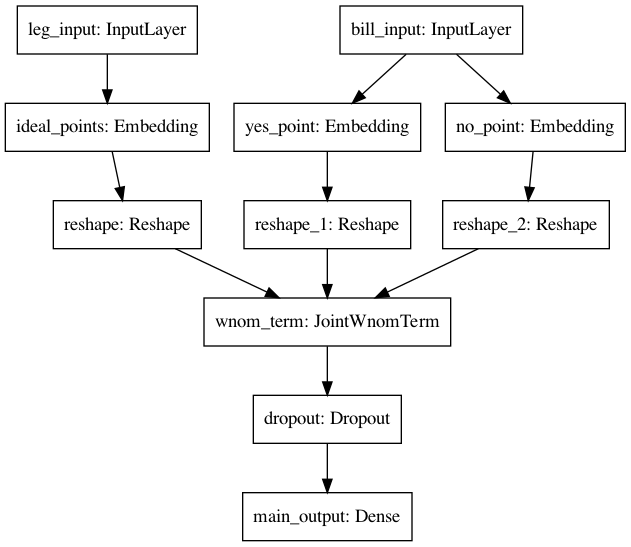
\includegraphics[width=0.75\linewidth]{model} 

}

\caption{\label{fig:model1}Base Model}\label{fig:unnamed-chunk-3}
\end{figure}

\begin{itemize}
\item
  Input layers: The inputs to this model consist of numeric ids for both
  legisators and bills. The data is given as a batch of triples,
  \((legislator\_id, bill\_id, vote)\).
\item
  Embedding layers: These layers take the numeric ids and convert them
  into continuous measures, for example mapping a specific legislator id
  to her ideal point. In this model there is one ideal point embedding
  for legislators, and two embedding for bills, the yes\_point and the
  no point, that correspond to numeric values associated with WNOMINATE
  style estimation. The ideal point layer is restricted in two ways.
  First, the model includes orthogonality regularization on the ideal
  points \citep{orthreg1, orthreg2}. This penalizes correlation between
  ideal point dimensions and ensures that the resulting estimates are
  orthogonal. Ideal point embeddings also have a maximum norm
  constraint, which ensures that the norm of the ideal point vector for
  any legislator lies within the unit hypersphere.\footnote{Note that
    the maximum norm constraint does not require that any legislator
    actually attain a unit norm. This differs somewhat from existing
    implementations which seem to ensure all dimensions fill the range
    from {[}-1, 1{]}. If this behavior is desired, it can be easily
    fixed in postprocessing.}
\end{itemize}

\begin{itemize}
\item
  Reshape layers: Because they are often used for text analysis, by
  default embedding layers assume that there is a sequence of ids to to
  transform into the embedding space. Since we have only a single id to
  embed, these layers drop the dimension associated with the sequence to
  form a two dimensional tensor.
\item
  JointWnomTerm layer: The embedded and reshaped data is fed into a
  custom neural network layer that implements the conventional WNOMINATE
  estimation (cite Poole and Rosenthal and the WNOMINATE package).
  Specifically, the layer implements the inner portion of model in
  \ref{eq:wnom}, sepcifically calculating

  \begin{equation} \label{eq:jointwnom}
  \exp\left(-\frac{1}{2}\sum_{k=1}^s w_k^2 d_{ijyk}^2 \right) - \exp\left({-\frac{1}{2}\sum_{k=1}^s w_k^2 d_{ijnk}^2 }\right)
  \end{equation}

  where \(K\) is the number of dimensions in the model, \(w_k\) is the
  salience weight for dimension \(k\), and \(d_{iyk}^2\) is the distance
  between a legislator's ideal point and the yes point of the bill and
  \(d_{ink}^2\) is the distance between the legislator's ideal point and
  the no point of the bill.{[}\^{}10{]}
\item
  Dropout layer: Dropout regularization, as proposed by \cite{dropout},
  has become an extremely common way of limiting model overfitting,
  often with the additional benefit of improved behavior during model
  training. Dropout layers set model weights to 0 at random during
  iterations of the training process. This prevents any single weight
  dominating the prediction of the algorithm. In this specific instance,
  the dropout layer sets the salience weight for any given ideology
  dimension to 0 for a specific iteration of the optimzation algorithm
  relying upon the other dimensions to make a vote prediction. In
  practice, this has resulted in better model performance in terms of
  observable metrics and by limiting overfitting during the training
  process..
\item
  Dense layer: The quantity obtained in the JointWnomLayer is then used
  as an input to a Dense layer, parameterised as a logistic regression
  (i.e.~sigmoid activation and binary\_crossentropy loss). The single
  model weight estimated here is denoted \(\beta\) in most NOMINATE
  models and represents the signal to noise ratio. A high value
  corresponds to votes being largely deterministic, a lower value
  suggest more randomness.
\end{itemize}

\section{The neural network implementation
works}\label{the-neural-network-implementation-works}

We demonstrate that the neural network implementation works at least as
well as existing methods through two simple tests. The first is to test
the model on synthetic data, generated with known parameters, and
determine how well the method recovers these known values. The second is
to check that the results match the commonly used implementations of
WNOMINATE \citep{wnominate} and item response \citep{pscl} ideal points.

\subsection{Recovering known ideal
points}\label{recovering-known-ideal-points}

The synthetic data is generated to have 3 known dimensions, where the
random predictions are generated in the NOMINATE parameterization. To
guard against overfitting to specific votes a legislator took, we train
the model on a subset of the data and test it on 20\% of votes as a held
out set. This means that a legislator's ideal point is determined only
by the votes in the training sample and that a bill's paramters are
determined only by the subset of legislators included who voted on this
bill.

There are two primary benefits to using a held out sample. First,
relying on an out of sample evaluation set is often used to determine
when a neural network has converged while estimating a model. There is
little point in continuing to optimize a model where out of sample
performance has plateaued and doing so usually results in overfitting.
Second, performance on a held out sample can be used to make additional
decisions about the model structure, including parameterization choices
or for evaluating distributional assumptions. For example, how does
making the ideal points dynamic affect the model performance? What is
the optimal number of ideal point dimensions? An additional dimension
may offer an improvement in out of sample prediction, but it almost
always increases in sample performance. The decision to add a dimension
has always been somewhat arbitrary, an out of sample performance test
provides an objective metric to evaluate.\footnote{It is not as simple
  as saying that ``the model that fits best on test data'' is the right
  answer. In some cases it is preferable to say, this is the first model
  that attains a near minimum.}

\begin{figure}

{\centering 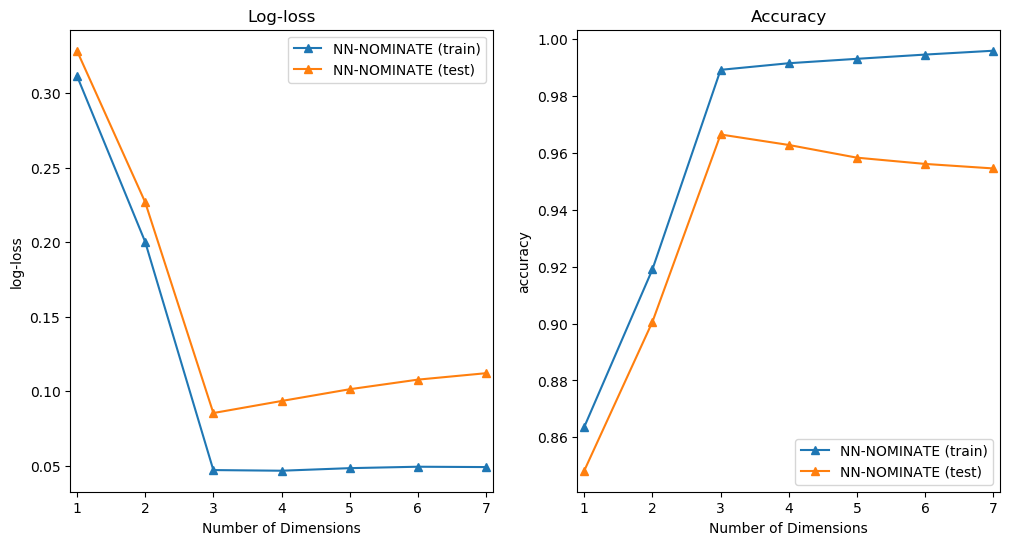
\includegraphics[width=1\linewidth]{test_metrics} 

}

\caption{\label{fig:testmetrics}Performance metrics on Synthetic Data}\label{fig:unnamed-chunk-4}
\end{figure}

Figure \ref{fig:testmetrics} shows the model performance of NN-NOMINATE
on synthetic data, varying the number of dimensions in the model. We
evaluate two metrics, accuracy (whether or not the vote was predicted
correctly) and log-loss (a common metric used in classification
problems). Log-loss is useful because it provides an idea of how good
the probability estimates of a model are, and penalizes over-confident
predictions. We see that the log-loss decreases rapidly is minimized at
the optimal number of dimensions on the test data, and the test log-loss
begins to increase even as in sample . Training accuracy shows similar
patterns, attaining best performance on the known optimal number of
dimensions.

\subsection{Comparison to existing
pacakges}\label{comparison-to-existing-pacakges}

\begin{figure}

{\centering 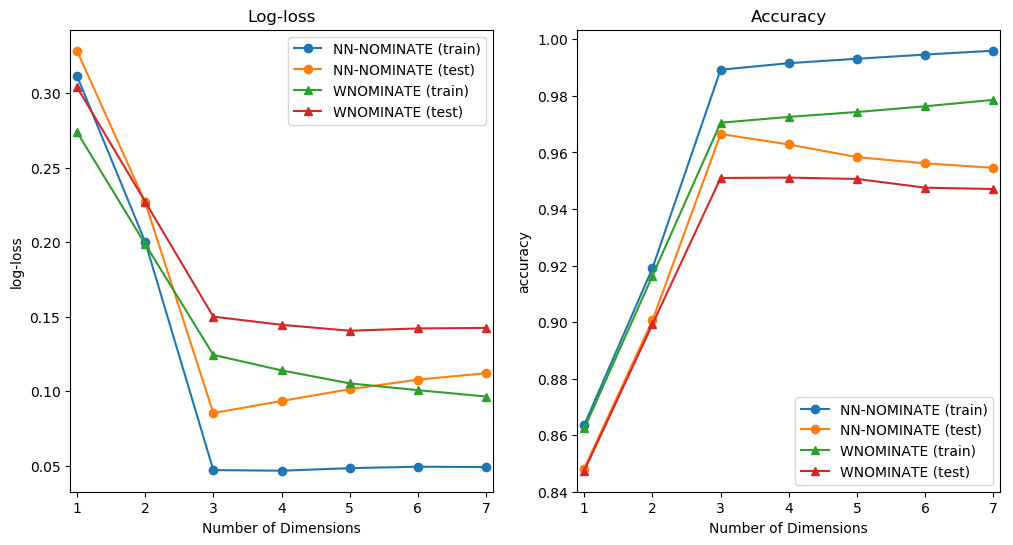
\includegraphics[width=1\linewidth]{test_metrics_with_wnom} 

}

\caption{\label{fig:testmetricswnom}Performance metrics on Synthetic Data}\label{fig:unnamed-chunk-5}
\end{figure}

Since is has not yet been common to estimate ideal point models on a
training and test set we verify that the model works by comparing the
results of NNNOMINATE to the WNOMINATE package available in R. The
results for the synthetic data are shown in Figure
\ref{fig:testmetricswnom}, where WNOMINATE shows similar patterns over
training and test data. It appears that for the synthetic dataset at
least, NN-NOMINATE (slightly) outperforms the commonly used WNOMINATE
package attaining lower log loss and higher accuracy on test data.

In Table XX, we show the same metrics on real world data from the
110th-115th US Senate. In addition to similar performance metrics, the
results of the two methods are strongly correlated.\footnote{Since ideal
  points are not independently identified, including up to dimension
  switching and other problems, we use simple correlations between the
  metrics as our outcome of choice. It is often the case that
  NN-NOMINATE results in ideal points that are smaller in maginitude on
  average than the WNOMINATE package.}

\begin{figure}

{\centering 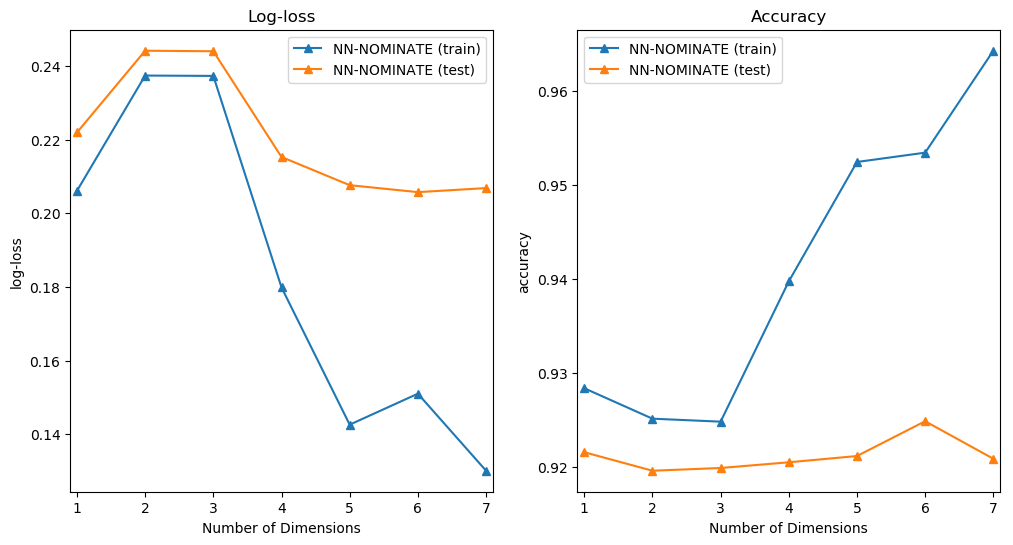
\includegraphics[width=0.75\linewidth]{votes_metrics} 

}

\caption{\label{fig:votesmetrics}Log-loss on 110th-115th Senate}\label{fig:unnamed-chunk-6}
\end{figure}

\section{Results and applications}\label{results-and-applications}

While it is comforting to know that a new optimization of an existing
model returns similar results, NN-NOMINATE is capable of more than the
existing implementations. The first is large scale ideal point
estimation, for example fitting models on the entire history of the US
Congress locally on a laptop. The second is to demonstrate the
extensibility of the framework, where the model can be extended very
simply to include covariates as well as more complicated representations
of a bill than existing representations.

\subsection{}\label{section}

We examine two large datasets, all of which can be fitted locally on a 3
year old mac laptop in less than an hour.\footnote{Formal performance
  comparisions to existing methods is forthcoming. Note that in the case
  of the WNOMINATE and pscl packages, performance comparisons are
  impossible because they require computaiton of a roll call matrix that
  is nXm which is more than can easily fit in memory (assuming integer
  values for all votes this still takes up more than XXGB).{]}} The
first is simply the entire history of US rollcalls. The dimension
tradeoff calculation from above is shown in Figure XX, which shows that
the optimal number of dimensions is at least 8 over this entire dataset.

The second dataset is the set of all cosponsorship decisions from the
93rd-114th US Congresses, a task that was also attempted in (cite that
earlier paper). While that work hypothesized that cosponsorship would
show fewer dimesions than voting, we believe that it is also plausible
that there should be more. Since so many voting decisions include
strategic concerns, cosponsorhip, a potentially less impactful choice,
could allow legislators to espouse a wider variety of policy opinions
(and thus require additional dimensions in the modeling process).

In this case, a ``yes'' vote is considered to be sponsoring or
cosponsoring a bill, whereas everyone who did not is assumed (at least
by opportunity cost) to be a ``no''. Note that this data is much noiser
than votes. Since so many bills are introduced that do not proceed in a
given session, there are likely many cases where a legislator would have
preferred that a bill pass even if they did not have the opportunity to
copsonsor it. Because of this, we add additional dropout layers on the
bill parameters themselves. This limits the extent to which the model
can overfit to noise in the dataset, although the results in Table XX
show that this is only somewhat successful as the training accuracy
somewhat rapidly reaches 1.

While the above results could be construed as evidence, as was the
assertion made (in that other paper), that there are fewer dimensions in
cosponsoring decisions than there are in voting it seems equally
plausible that the model is more easily fitting to noise in the
cosponsorship decisions so rapidly that the true policy preference
dimensions.

\subsection{}\label{section-1}

We also extend the model to include a simple covariate. It is plausible
that a legislator might behave differently while in the party that
controls the chamber. One way this might be observerd is that a
legislator in the party in power is more likely to vote yes, on average,
than someone in the minority party. This could even be the case when the
match with their ideal point is very close, but due to party pressure a
legislator could deviate from this to some extent. As such we estimate
the models from the previous section including a variable indicating
that a legislator is in the party in power so that the logistic layer
now becomes:

\begin{equation}
prob(vote=yea) = \Phi\left(\beta \left[\exp\left(-\frac{1}{2}\sum_{k=1}^s w_k^2 d_{iyk}^2 \right) - \exp\left({-\frac{1}{2}\sum_{k=1}^s w_k^2 d_{ink}^2 }\right)\right] + \gamma * pip_{ik}\right)
\end{equation}

where \(\gamma\) represents the effect of being in the party in power.
The results show that this factor is positive, as expected, but that the
magnitude represents only a very small difference in vote probability.
Note that the NN-Nominate framework does not easily lend itself to
hypothesis testing. One way to achieve this would be a parametric
bootstrap (ala Poole and Rosenthal) but this has not been
attempted.\footnote{Blei paper about neural networks as Bayesian
  inference.}

Additionally, while a discussion of using a text representation of a
bill, rather than a simple indicator value, is beyond the scope of this
work this is a prime area of current research (see e.g.~Kornilova).
These models work by building embedding representations of the bills
themselves and then determining legislators ideal points relative to
this more robust representation of a bill. While the accuracy of these
models does not yet match that of the bill indicator approach, these
models have the strong advantage of allowing out of sample prediction on
new bill text. This means that we can determine how a legislator would
vote on new bills, as they are introduced (for more we refer you to the
Kornilova paper).

\section{Conclusion}\label{conclusion}

\begin{enumerate}
\def\labelenumi{\arabic{enumi}.}
\tightlist
\item
  I implemented DW-NOMINATE as a neural network

  \begin{itemize}
  \tightlist
  \item
    Why? Because I could! But also because it's a nice platform for this
    kind of optimization.
  \item
    It scales much better than existing implementations
  \item
    It's extensible in very interesting ways
  \end{itemize}
\item
  All ideal point models are (a bit) overfit.

  \begin{itemize}
  \tightlist
  \item
    At some point the algorithm starts to make marginal improvements to
    the parameters that don't improve out of sample performance
  \item
    Out of sample performance matters much more than in sample (e.g.~if
    we only cared about in sample we'd just add dimensions until we cam
    predict it perfectly)
  \item
    Out of sample performance is a useful metric for evaluating modeling
    choices (adding another dimension, adding a time component, adding
    an external variable)
  \end{itemize}
\end{enumerate}

this is inline 42 and

\begin{Shaded}
\begin{Highlighting}[]
\NormalTok{py}\OperatorTok{$}\NormalTok{answer}
\end{Highlighting}
\end{Shaded}

\begin{verbatim}
## [1] "42"
\end{verbatim}

\begin{enumerate}
\def\labelenumi{\arabic{enumi}.}
\tightlist
\item
  How to implement in a neural network

  \begin{enumerate}
  \def\labelenumii{\alph{enumii}.}
  \tightlist
  \item
    Discuss both parameterizations
  \item
    Show convergence plots
  \item
    Discuss out of sample fit as the metrics of importance
  \end{enumerate}
\item
  A Neural Network implementation works

  \begin{enumerate}
  \def\labelenumii{\alph{enumii}.}
  \tightlist
  \item
    It estimates correctly on synthetic data (accuracy tables for both
    of these)
  \item
    It matches results from standard libraries (wnominate and pscl) on
    both synthetic and real data

    \begin{enumerate}
    \def\labelenumiii{\roman{enumiii}.}
    \tightlist
    \item
      Show both in sample and out of sample accuracy (will require
      writing a python wrapper to get predictions from the R results)
    \end{enumerate}
  \end{enumerate}
\item
  Results and applications of the neural network implementation

  \begin{enumerate}
  \def\labelenumii{\alph{enumii}.}
  \tightlist
  \item
    What are the optimal number of dimensions? Plot these and discuss
    tradeoffs
  \item
    Applying the model to cosponsorship
  \item
    Polarization differences

    \begin{enumerate}
    \def\labelenumiii{\roman{enumiii}.}
    \tightlist
    \item
      Votes models over time (how to do in multiple dimensions?)
    \item
      Compare between cosponsorship and votes
    \end{enumerate}
  \end{enumerate}
\end{enumerate}

Dropout in two places: 1. Each dimension to ensure fitting even if first
dimensions dominates. 2. On bill embeddings (to not overfit to a
specific bill). Why not on legislators? The structure of the dynamic
part of the model doesn't allow this easily.




\newpage
\singlespacing 
\bibliography{nnnominate.bib}

\end{document}
